\documentclass[12pt]{article}

\usepackage[margin=1in]{geometry}
\usepackage{graphicx}

\begin{document}
	
	\noindent Jacob Hendricks \\ Thesis Proposal
	
	\section*{Introduction}
	Scheduling of processes is an important function of an operating system.
	It must be fair, such that every process has a chance at time on the CPU.
	It must be responsive, such that interactive processes, those being marked by high levels of I/O operations, can be sufficiently responsive according to the desires of users.
	It must be light weight so that as little time as possible is spent on scheduling of processes so that as much time as possible can be spent on the processes themselves.
	
	Proposed here is a novel scheduling algorithm called the Prime-Mod Scheduler, so named because of the core functionality of using prime numbers and the modulus operation to determine which queue to draw a process from to get time on the CPU.
	The Prime-Mod Scheduler is a kind of hybrid between a priority queue scheduler and a lottery scheduler.
	
	\section*{How the Prime-Mod Scheduler Works}
	There are a number of queues, and each queue has a prime number assigned to it, starting with 2 and continuing in ascending order until all queues have a prime number assigned to it.
	A counter, initialized at 0 on system start up, is incremented at the start of every invocation of the scheduler. 
	That number is then modded by the prime number of each queue until the result is 0.
	If that queue has a process in it, then the process at the front of the queue is chosen to be ran.
	If that queue does not have a process in it, then the process on the front of the highest priority queue with a process in it is chosen instead.
	If a process yields time early because of waiting on I/O, then that process will be promoted to the next highest priority queue.
	If a process uses all of its allotted time, then the process will be demoted to the next lowest priority queue.
	If the invocation counter does not mod evenly by any of the prime numbers assigned to the queues, then the highest priority queue is chosen.\\
	
	
	Each priority queue comprises two sub-queues - the front-half and the back-half.
	The front-half consists of processes that entered the queue from a lower priority queue while the back-half consists of processes that entered the queue from a higher priority queue.
	New processes are entered at the back of the front-half of the highest priority queue, so the highest priority queue will have no back-half sub-queue. \\
	
	Newly created processes will enter at the back of the front-half of the highest priority queue.
	
	\begin{center}
		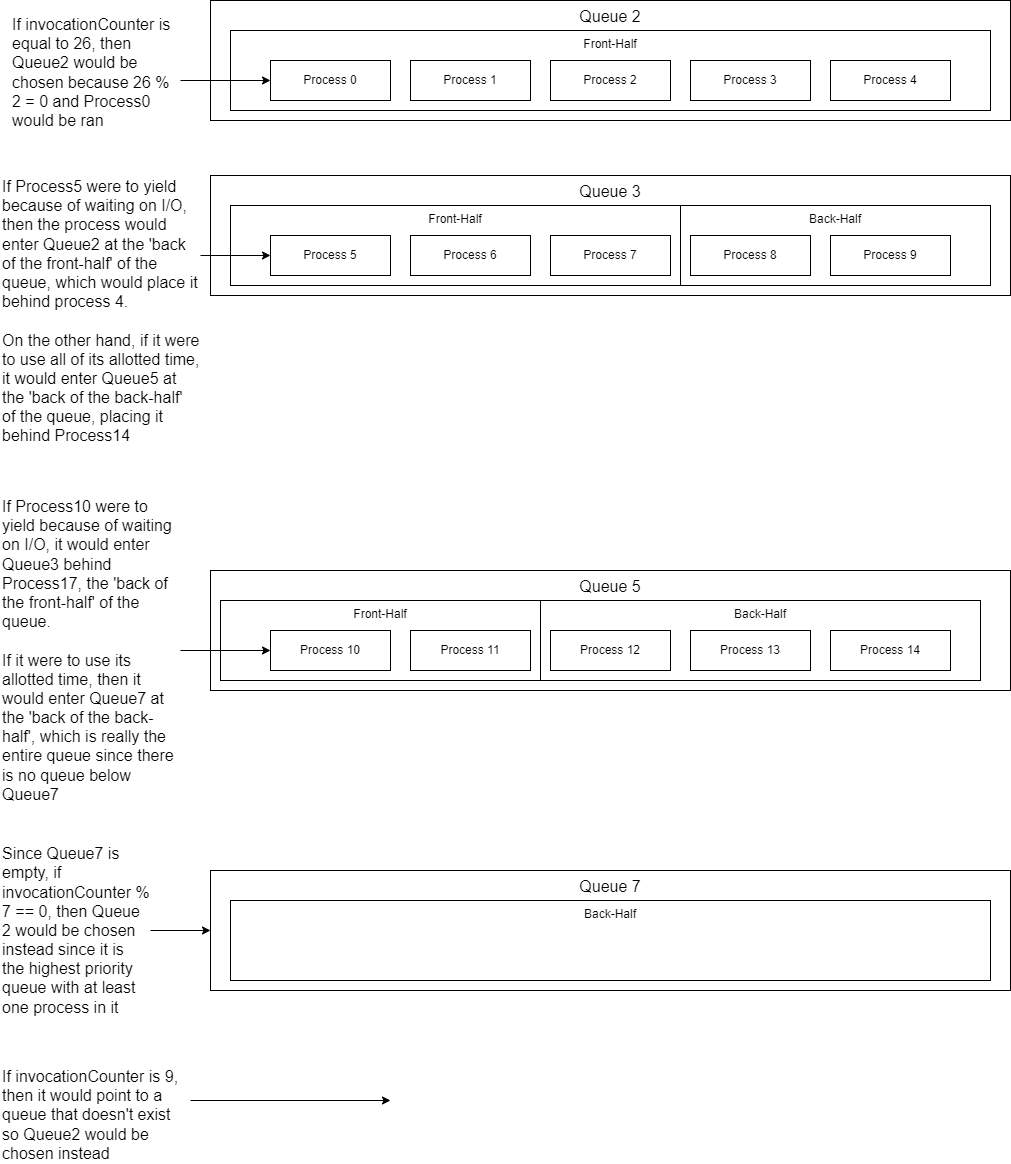
\includegraphics[scale=.45]{./diagram.png}
	\end{center}
	
	\section*{Work to be Done}
	In order to evaluate the effectiveness of the Prime-Mod Scheduler against other existing scheduling algorithms, a scheduling test bench application will be created.
	All of the popular and well known scheduling algorithms will be implemented and ran in this test bench: Round Robin, Priority Queue, Completely Fair Scheduler, Prime-Mod Scheduler, along with others yet to be added to this list.
	Their responsiveness will be measured, that is the amount of time it takes for a process to be rescheduled after it has waited for I/O operations to complete, and compared.
	Their time complexity execution will be derived and compared.
	The total time of execution of each process will be measured and compared.
	The fairness will be determined and compared.\\
	
	In order to achieve this, time will be normalized as 'CPU cycles'.
	Sets of artificial processes will be created.
	A process will comprise a total run execution time, a series of I/O wait operations which prescribe at what point the I/O wait will happen and how long it will last.
	The test bench application will take the sets and run them through the scheduler and capture the above mentioned values.
		
\end{document}